\documentclass[tikz]{standalone}
\usepackage{tikz}
\usetikzlibrary{positioning, graphs}
\usetikzlibrary{graphs.standard}
\begin{document}
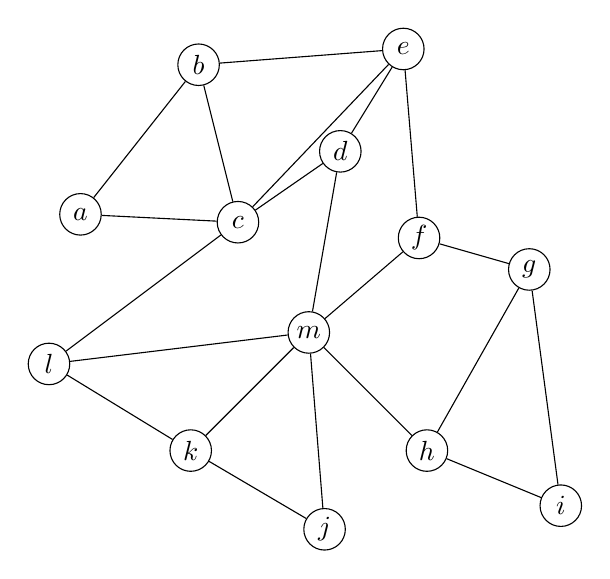
\begin{tikzpicture}
    [mynode/.style={draw,circle,inner sep = 0em, minimum size = 15}]
    \node[mynode] (a) at ( 0.0, -0.4) {$a$};
    \node[mynode] (b) at ( 1.5,  1.5) {$b$};
    \node[mynode] (c) at ( 2.0, -0.5) {$c$};
    \node[mynode] (d) at ( 3.3,  0.4) {$d$};
    \node[mynode] (e) at ( 4.1,  1.7) {$e$};
    \node[mynode] (f) at ( 4.3, -0.7) {$f$};
    \node[mynode] (g) at ( 5.7, -1.1) {$g$};
    \node[mynode] (h) at ( 4.4, -3.4) {$h$};
    \node[mynode] (i) at ( 6.1, -4.1) {$i$};
    \node[mynode] (j) at ( 3.1, -4.4) {$j$};
    \node[mynode] (k) at ( 1.4, -3.4) {$k$};
    \node[mynode] (l) at (-0.4, -2.3) {$l$};
    \node[mynode] (m) at ( 2.9, -1.9) {$m$};
    
    \draw (a) -- (b);
    \draw (a) -- (c);
    \draw (b) -- (c);
    \draw (b) -- (e);
    \draw (c) -- (d);
    \draw (c) -- (e);
    \draw (c) -- (l);
    \draw (d) -- (e);
    \draw (d) -- (m);
    \draw (e) -- (f);
    \draw (f) -- (g);
    \draw (f) -- (m);
    \draw (g) -- (h);
    \draw (g) -- (i);
    \draw (h) -- (i);
    \draw (h) -- (m);
    \draw (j) -- (m);
    \draw (j) -- (k);
    \draw (k) -- (m);
    \draw (k) -- (l);
    \draw (l) -- (m);

    % \draw (e) .. controls (7, 1) and (7, -3) .. (i);
    % \draw (a) .. controls (-3, -2) and (1.5, -6) .. (j);
    % \draw (f) -- (j);
    % \draw (b) -- (k);
    % \draw (d) .. controls (3.5, -2.2) and (4.5, -2) .. (i);
    % \draw (e) .. controls (3.5, -2.2) and (4.5, -2) .. (h);
    % \draw (c) .. controls (2.2, -1.8) and (2.2, -2.1) .. (j);

\end{tikzpicture}
\end{document}